
\begin{exercise}
% !TEX root = ../main.tex


\pt{4}\begin{minipage}[t]{.6\linewidth}
	Teken de overeenkomstige $x(t)$- en $a(t)$-grafiek bij de gegeven $v(t)$-grafiek. Ga ervan uit dat $x_0=\SI{0}{m}$.
\end{minipage}
\hfill
\begin{minipage}[t]{.37\linewidth}
	\raisebox{1ex-\height}{%
		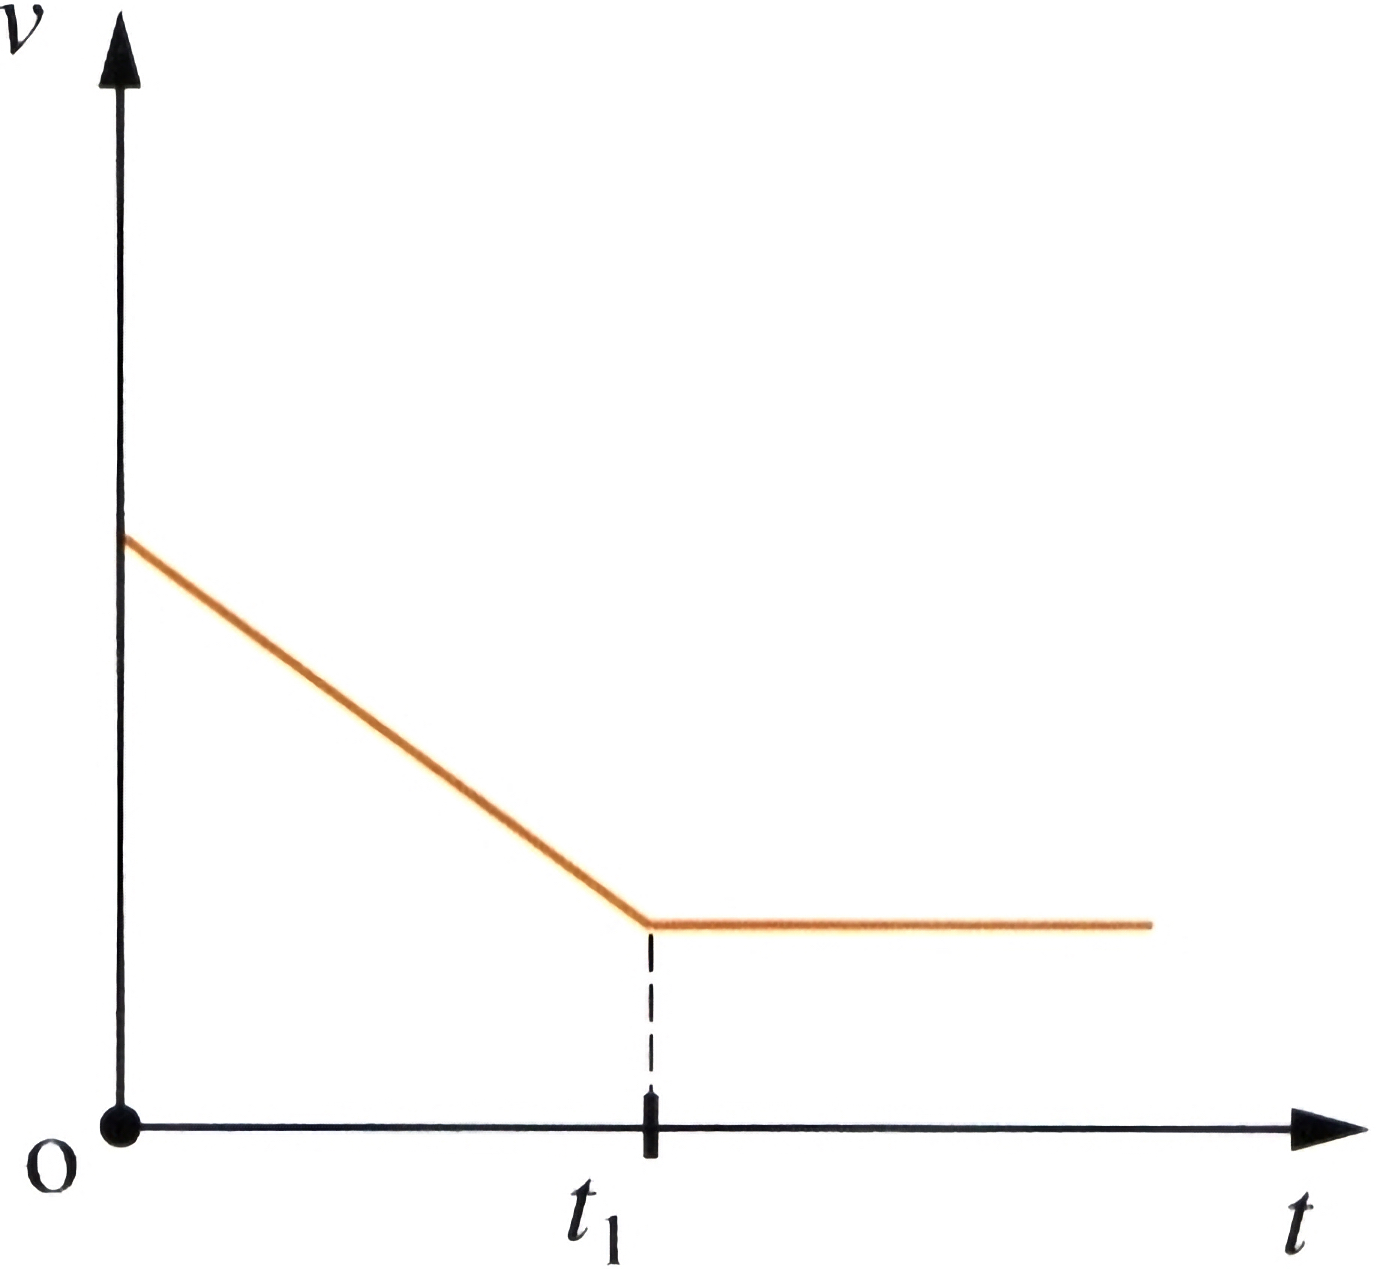
\includegraphics[width=\textwidth]{v(t)}%
		} 
\end{minipage}

\end{exercise}
